\chapter{Теоремы о промежуточных значениях непрерывной функции.}
\section{Теоремы о промежуточных значениях непрерывной функции}

\begin{thm} [о промежуточных значениях] \label{ch3n2}
Пусть функция $f$ непрерывна на отрезке $\Delta$ и принимает значения $A,B \in \bbR$ в точках $a$ и $b$ соответственно. Тогда для любого $C\in[A,B]$ существует такая точка $\xi \in [a,b]$, что $f(\xi)=C$.
\end{thm}
\begin{proof}
По условию, в $\Delta$ существуют точки $a$ и $b$ такие, что $f(a) = A$, $f(b) = B$. Если, например, $a < b$, то $[a; b]\in \Delta$.
Через $c_1$ обозначим середину отрезка $[a;b]$. Если $f(c_1) = C$, то утверждение доказано.

Пусть $f(c_1)\ne C$. Тогда, если $f(c_1) > C$, то положим $a_1 = a$, $b_1 = c_1$, а если $f(c_1) < C$, то $a_1 = c_1$, $b_1 = b$, и поэтому всегда $f(a_1)<C<f(b_1)$.

Отрезок $[a_1; b_1]$ снова разделим пополам, и через $c_2$ обозначим его середину. Если $f(c_2) = C$, то утверждение доказано. Если же $f(c_2) \ne C$, то через $[a_2;b_2]$ обозначим ту половину, для которой $f(a_2) < C < f(b_2)$, и т.д. Процесс или обрывается на некотором шаге, и тогда утверждение доказано, или получается последовательности вложенных отрезков $[a_n;b_n]$ таких, что $\lim_{n \to \infty}\limits(b_n-a_n)=0$ и
$$
f(a_n)<C<f(b_n) \fa n\in \bbN.
$$

По \hyperref[exp3]{теореме о стягивающихся отрезках} $\exists!\; c \in \bigcap_{n \in \bbN}\limits[a_n;b_n] \Rightarrow c\in [a;b]$, причем 
$$
\lim_{n \to \infty}a_n = \lim_{n \to \infty}b_n = c \fa n \in \bbN
$$

Согласно условию Гейне непрерывности функции $f$ в точке $c\in[a;b]$:
$$
\lim_{n \to \infty}f(a_n) = \lim_{n \to \infty}f(b_n) = f(c) \fa n \in \bbN,
$$

Из $f(a_n)<C<f(b_n) \fa n\in\bbN$ следует 
\begin{equation*}
\begin{split}
\lim_{n \to \infty}f(a_n) &\le C \le \lim_{n \to \infty}f(b_n),\\
f(c)&\le C\le f(c).\\
\end{split}
\end{equation*}

Из приведенных выше неравенств $f(c)=C$.

Случай, когда $a > b$, рассматривается аналогично. 

\noindent 
Теорема доказана.
\end{proof}
Эту теорему можно сформулировать следующим образом:	\textit{Если функция
$f$ непрерывна на промежутке $\Delta$, то множество $\Delta$ является промежутком.}

Заметим, что обратное утверждение является неверным, например, $f(x)= \sin(1/x)$ для $x\ne0$ и $f(0) = 0$ разрывна в точке $x = 0$, но у нее образ любого отрезка есть отрезок. Однако, что для монотонных функций обратное утверждение является верным.
\begin{defn}
Функция $f$ называется \textit{монотонно возрастающей (убывающей) на множестве} $X \in D_f$, если для любых $x_1$ и $x_2>x_1$ из множества $X$ 
$$
f(x_1)\le f(x_2) \quad (\text{соотв.}, f(x_1)\ge f(x_2)).
$$  
\end{defn}

\begin{defn}
Пусть $x_0$ --- точка разрыва функции $f$. Тогда 
\begin{enumerate}
\item
%\begin{figure}[!h]
%\centering
%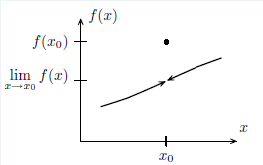
\includegraphics[width=0.7\textwidth]{pictures/pict2}
%\end{figure}
%(что-то сделать с картинкой надо будет)

Если $\exists \lim_{x \to x_0}\limits f(x) \in \bbR$, то $x_0$ - \textit{точка устранимого разрыва}
\item
Если $\exists \lim_{x \to x_0\pm0}\limits f(x)=f(x_0\pm 0)$, но $f(x_0+0)\ne f(x-0)$, то $x_0$ -- \textit{точка разрыва первого рода}, а число $\Delta f=f(x_0+0)-f(x_0-0)$.
\item
Все другие точки разрыва называют \textit{точками разрыва второго рода.}(т.е. хотя бы один из односторонних пределов либо не существует, либо бесконечен).
\end{enumerate}
\end{defn}
\begin{thm} \label{ch3n1} (\textbf{пока непонятно что делать, но это яковлев 90})
Если функция $f(x)$ определена и монотонна на интервале $(a;b)$, то в каждой точке $x_0\in(a;b)$ она имеет односторонние пределы. Причем, если $f(x)$ -- возрастающая, то 
$$
f(x_0-0)\le f(x_0)\le f(x_0+0),
$$
а если убывающая, то
$$
f(x_0-0)\ge f(x_0)\ge f(x_0+0).
$$
\end{thm}
\begin{thm}
Если функция $f$ определена и монотонна на промежутке $\Delta$ и $f(\Delta)$ — промежуток, то $f$ непрерывна на $\Delta$.
\end{thm}
\begin{proof}
Предположим противное, что функция $f$ разрывна в точке $x_0 \in\Delta$. Тогда по Теореме \ref{ch3n1} в точке $x_0$ обязательно существуют односторонние пределы, значит $x_0$ не является точкой разрыва второго рода.  А в случае устранимой точки разрыва $f(x_0-0)=f(x_0+0)$, т.е. отсюда и из неравенств из теоремы  \ref{ch3n1}, получим $f(x_0)=f(x_0-0)=f(x_0+0)$, т.е. функция непрерывна в точке разрыва, что невозможно. Значит $x_0$ не может быть точкой устранимого разрыва. Поэтому из монотонности следует, что $x_0$ может быть только точкой разрыва первого рода. Пусть, например, $f(x_0-0)\ne f(x_0)$.

Тогда $f$ не принимает значения, лежащие между $f(x_0 - 0)$ и $f(x_0)$, и поэтому $f(\Delta)$ не является промежутком, что противоречит условию. Следовательно, $f(x_0-0) = f(x_0)$. Аналогично доказывается, что  $f(x_0 + 0) = f(x_0)$, если, конечно, $x_0$ не является правым концом промежутка $\Delta$. 

\noindent
Теорема доказана.
\end{proof} 

\begin{thm}
Если функция $f$ непрерывна на отрезке $\Delta$, то $f(\Delta)$ — отрезок.
\end{thm}
\begin{proof}
Согласно теореме \ref{ch1n1} Вейерштрасса из прошлого билета 
\begin{gather*}
\exists x_* \in \Delta:\quad f(x_*)=m=\inf(f(\Delta)),\\
\exists x^* \in \Delta:\quad f(x^*)=M=\sup(f(\Delta)).
\end{gather*}   
Cогласно теореме \ref{ch3n2} о промежуточных значениях $f(\Delta)$ -- промежуток $\Rightarrow f(\Delta)=[m,M]$ 
\noindent
Теорема доказана.
\end{proof} 

Таким образом, при непрерывном отображении образом отрезка всегда является отрезок. Однако, как показывают примеры, образом интервала может быть любой промежуток.
